% #############################################################################
% This is Chapter 5
% !TEX root = ../main.tex
% #############################################################################
% Change the Name of the Chapter i the following line
\fancychapter{This is the Fifth Chapter}
\cleardoublepage
% The following line allows to ref this chapter
\label{chap:evaluation}

Lorem ipsum dolor sit amet, consectetuer adipiscing elit. Morbi commodo, ipsum sed pharetra gravida, orci magna rhoncus neque, id pulvinar odio lorem non turpis. Nullam sit amet enim. Suspendisse id velit vitae ligula volutpat condimentum. Aliquam erat volutpat. Sed quis velit. Nulla facilisi. Nulla libero. Vivamus pharetra posuere sapien. Nam consectetuer. Sed aliquam, nunc eget euismod ullamcorper, lectus nunc ullamcorper orci, fermentum bibendum enim nibh eget ipsum. Donec porttitor ligula eu dolor. Maecenas vitae nulla consequat libero cursus venenatis. Nam magna enim, accumsan eu, blandit sed, blandit a, eros. 
% #############################################################################
\section{Maecenas vitae nulla consequat} 
Aliquam aliquet, est a ullamcorper condimentum, tellus nulla fringilla elit, a iaculis nulla turpis sed wisi. Fusce volutpat. Etiam sodales ante id nunc. Proin ornare dignissim lacus. Nunc porttitor nunc a sem. Sed sollicitudin velit eu magna. Aliquam erat volutpat. Vivamus ornare est non wisi. Proin vel quam. Vivamus egestas. Nunc tempor diam vehicula mauris. Nullam sapien eros \Cref{fig:test_env}, facilisis vel, eleifend non, auctor dapibus, pede.

\begin{figure}[h]
\centering
\includegraphics[width=0.8\textwidth]{./Images/test_env}
\caption{Test Environment}
\label{fig:test_env}
\end{figure}

Aliquam aliquet, est a ullamcorper condimentum, tellus nulla fringilla elit, a iaculis nulla turpis sed wisi. Fusce volutpat. Etiam sodales ante id nunc. Proin ornare dignissim lacus. Nunc porttitor nunc a sem. Sed sollicitudin velit eu magna. Aliquam erat volutpat. Vivamus egestas. Nunc tempor diam vehicula mauris. Nullam sapien eros, facilisis vel, eleifend non, auctor dapibus, pede \Cref{tab:network_profiles} used in the tests. The Network Link Conditioner allows to force/simulate fluctuations in fixed network segments.

\begin{table}[htb]
\centering
\normalsize
    \caption{Network Link Conditioner Profiles}
    \label{tab:network_profiles}
{\footnotesize
    \begin{tabular}{ | c | c | c | c | }
    \hline 
    \textbf{Network Profile}	& \textbf{Bandwidth} & \textbf{Packets Droped} & \textbf{Delay}\\ \hline \hline
    Wifi  & 40 mbps  &  0\%  &   1 ms \\ \hline
    3G  & 780 kbps  &  0\%  &   100 ms \\ \hline 
    Edge  & 240 kbps  &  0\%  &   400 ms \\ \hline
    \end{tabular}
    }
\end{table}

Aliquam aliquet, est a ullamcorper condimentum, tellus nulla fringilla elit, a iaculis nulla turpis sed wisi. Fusce volutpat. Etiam sodales ante id nunc. Proin ornare dignissim lacus. Nunc porttitor nunc a sem. Sed sollicitudin velit eu magna. Aliquam erat volutpat. Vivamus ornare est non wisi. Proin vel quam. Vivamus egestas. Nunc tempor diam vehicula mauris. Nullam sapien eros, facilisis vel, eleifend non, auctor dapibus, pede.
% #############################################################################
\section{Proin ornare dignissim lacus}
Pellentesque habitant morbi tristique senectus et netus et malesuada fames ac turpis egestas. Vestibulum tortor quam, feugiat vitae, ultricies eget, tempor sit amet, ante. Donec eu libero sit amet quam egestas semper. Aenean ultricies mi vitae est. Mauris placerat eleifend leo. Quisque sit amet est et sapien ullamcorper pharetra. Vestibulum erat wisi, condimentum sed, commodo vitae, ornare sit amet, wisi. Aenean fermentum, elit eget tincidunt condimentum, eros ipsum rutrum orci, sagittis tempus lacus enim ac dui. Donec non enim in turpis pulvinar facilisis. Ut felis.

Et ``optimistic'' nulla dui purus, eleifend vel, consequat non, dictum porta, nulla. Duis ante mi, laoreet ut, commodo eleifend, cursus nec, lorem. Aenean eu est. Etiam imperdiet turpis. Praesent nec augue. Curabitur ligula quam, rutrum id, tempor sed, consequat ac, dui $G_j$, nec ligula et lorem consequat ullamcorper $p$ ut mauris eu mi mollis luctus $j$, porttitor ut, \Cref{unchoke_gain}, uctus posuere justo:

\begin{description}
  \item[$N_j$] Is the number of times peer $j$ has been optimistically unchoked.
  \item[$n_j$] Among the $N_j$ unchokes, the number of times that peer $j$ responded with unchoke or supplied segments to peer $p$.
  \item[$C_{r[j]}$] The cooperation ratio of peer $j$. If peer $j$ never supplied peer $p$, the information of $C_{r[j]}$ may not be available.
  \item[$C_{r (max)}$] The maximum cooperation ratio of peer $p$’s neighbors, i.e., $C_{r (max)} = max(C_r)$.
\end{description}

\begin{equation}
\label{unchoke_gain}
 G_j =
  \begin{dcases}
    \frac{n_j C_{r[j]}}{N_j} &\quad \text{if } n_j > 0\\
    \frac{C_{r (max)}}{N_j + 1} &\quad \text{if } n_j = 0
  \end{dcases}
\end{equation}

Cursus $C_{r (max)}$ conubia nostra, per inceptos hymenaeos $j$ gadipiscing mollis massa $N_j = 0$, unc ut dui eget nulla venenatis aliquet $G_j = C_{r (max)}$.

Vestibulum accumsan eros nec magna. Vestibulum vitae dui. Vestibulum nec ligula et lorem consequat ullamcorper. Class aptent taciti sociosqu ad litora torquent per conubia nostra, per inceptos hymenaeos. Phasellus eget nisl ut elit porta ullamcorper. Maecenas tincidunt velit quis orci. Sed in dui. Nullam ut mauris eu mi mollis luctus. Class aptent taciti sociosqu ad litora torquent per conubia nostra, per inceptos hymenaeos. Sed cursus cursus velit. Sed a massa. 

Both \Cref{fig:tx_layer_4,fig:tx_layer_5} Phasellus eget nisl ut elit porta ``perfect'' tincidunt. Class aptent taciti sociosqu ad litora torquent per conubia nostra.

\begin{figure}[h]
%\centering
       \subfigure[Adaptation System Test 4]{\label{fig:tx_layer_4}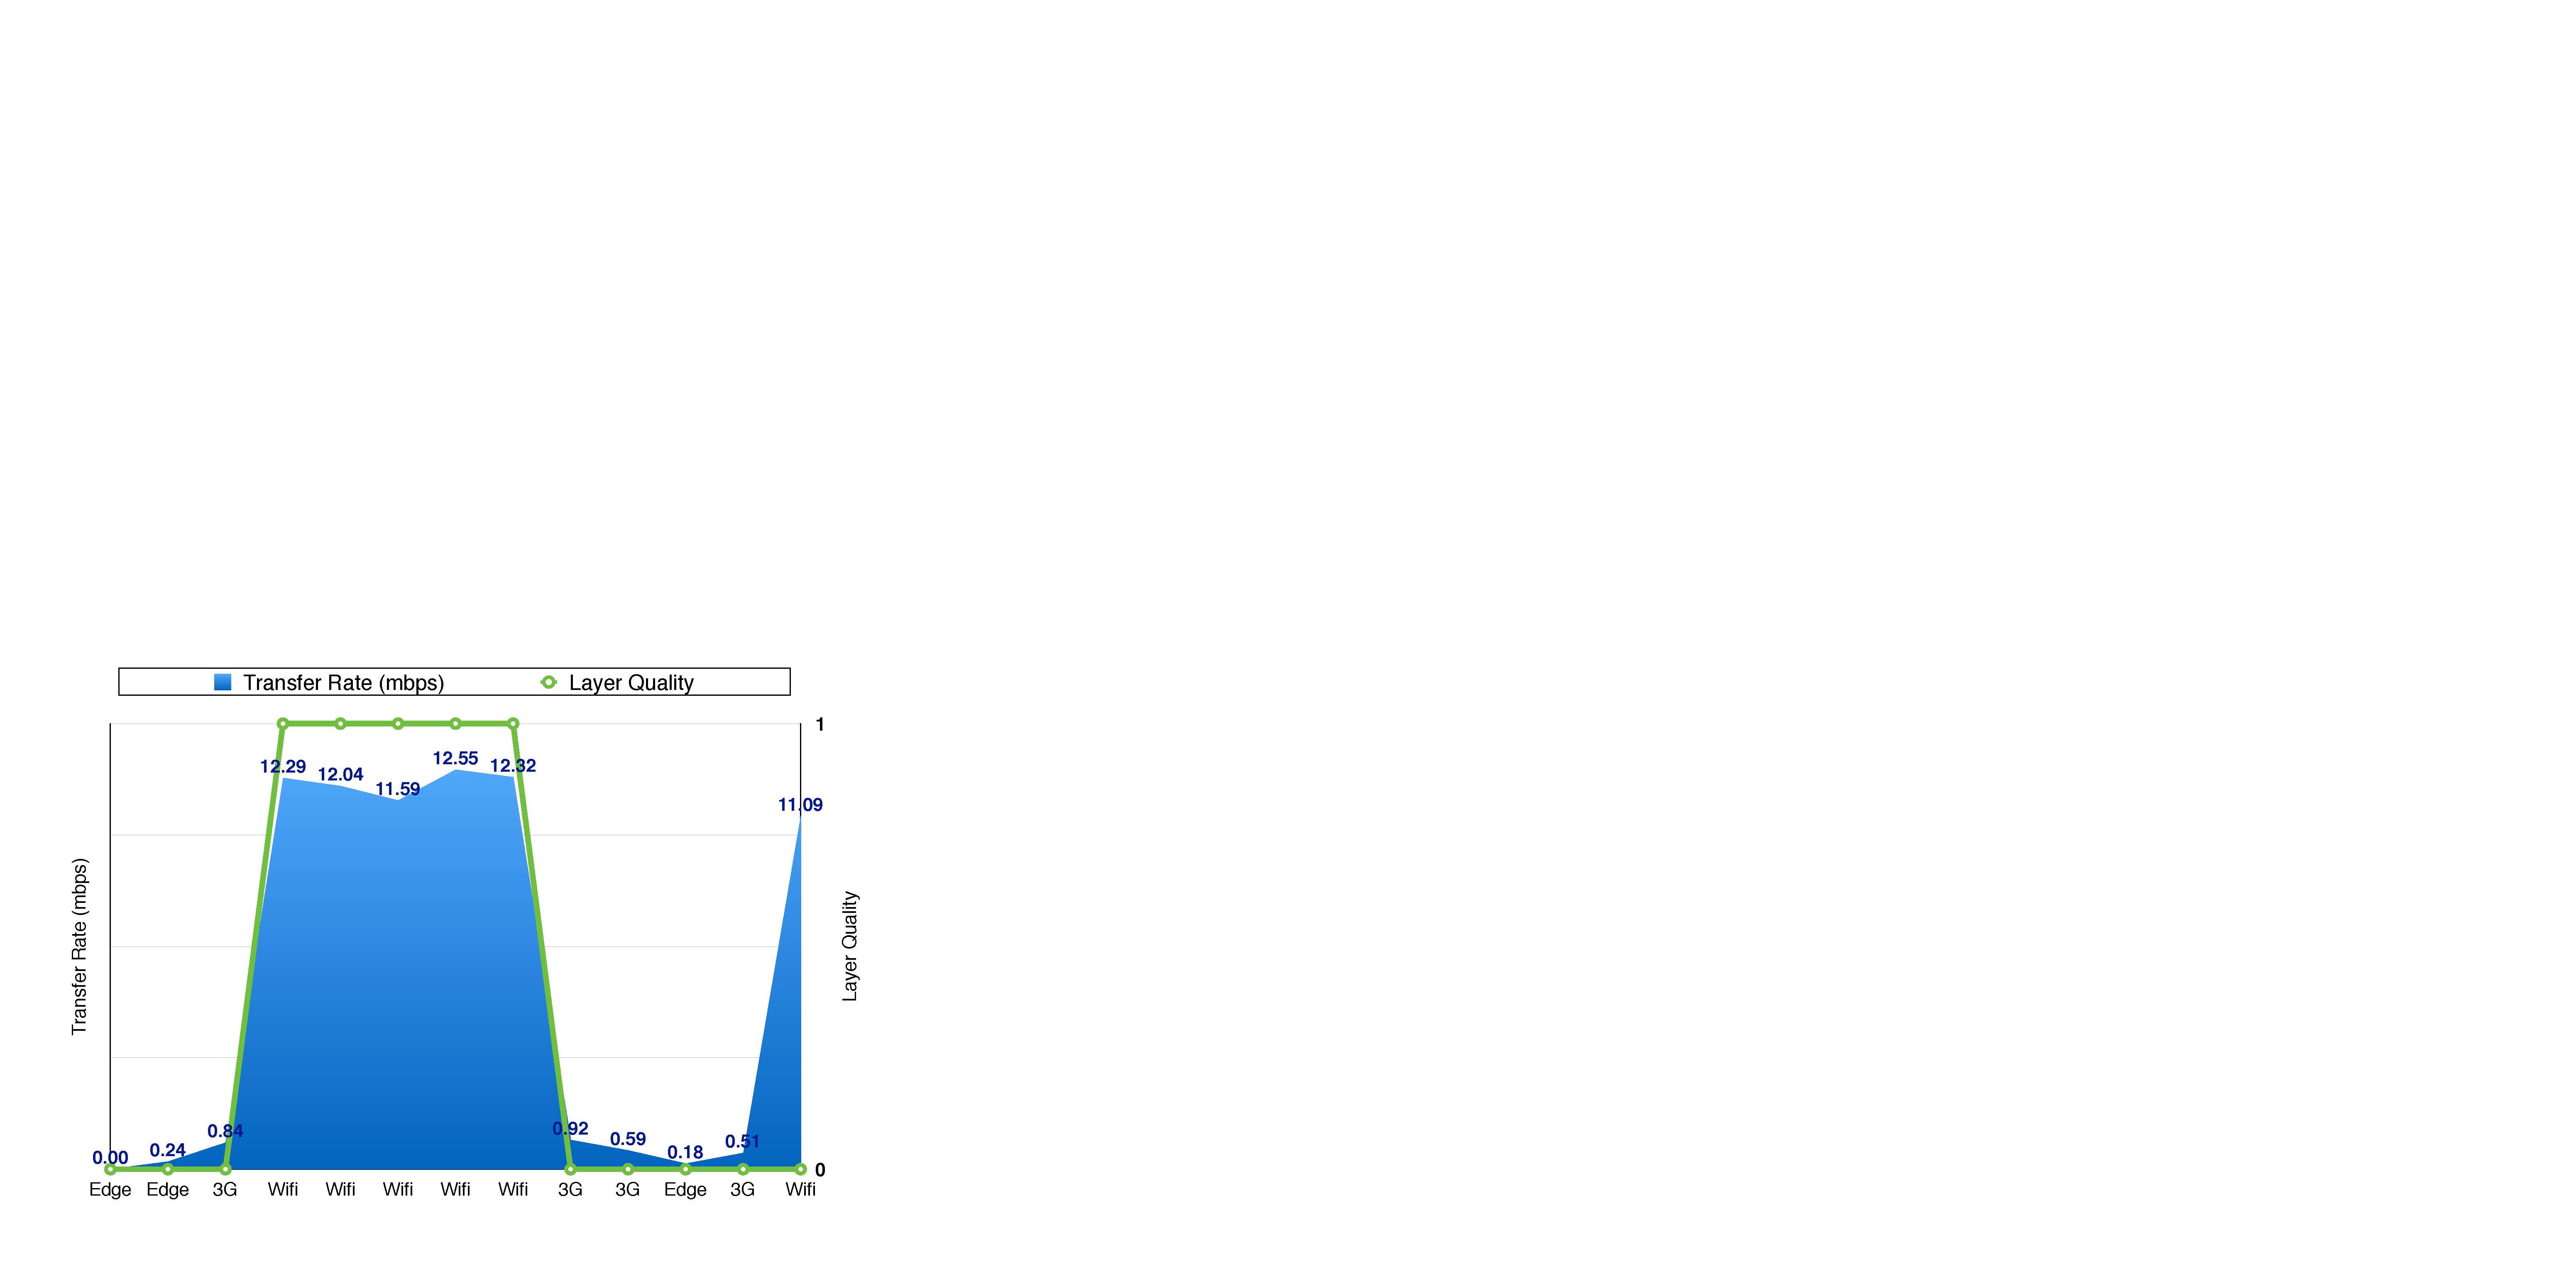
\includegraphics[width=0.5\textwidth]{./Images/tx_layer_4}}  
   %    \centering 
       \subfigure[Adaptation System Test 5]{\label{fig:tx_layer_5}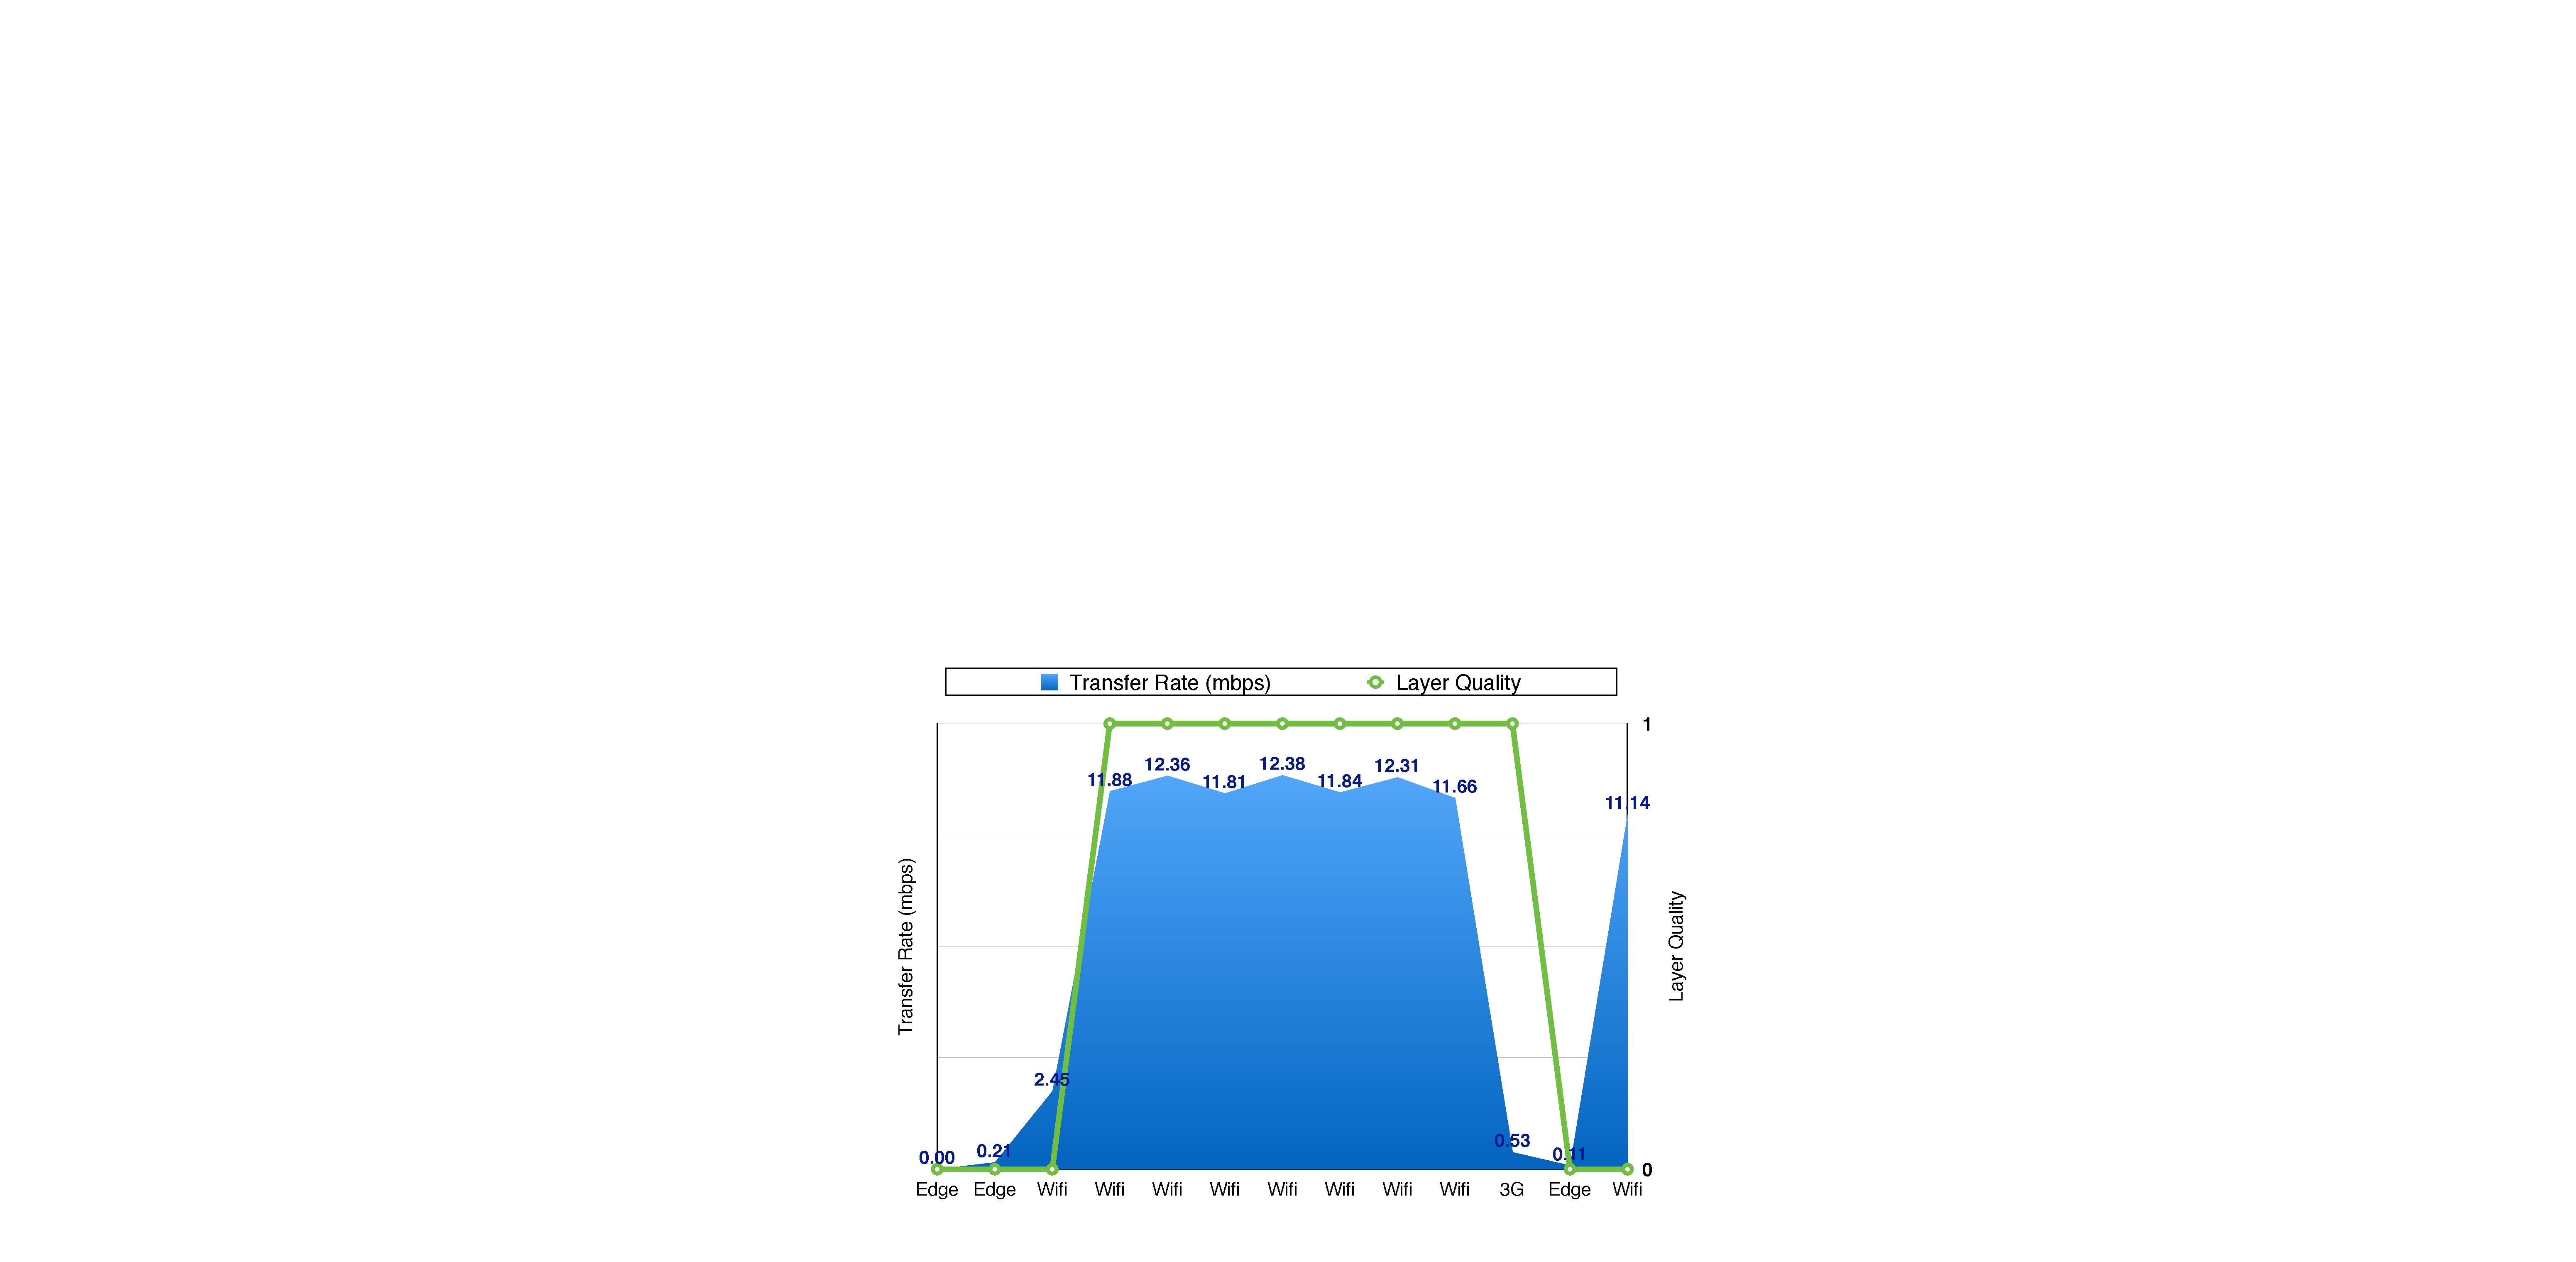
\includegraphics[width=0.5\textwidth]{./Images/tx_layer_5}}   
        \caption{Adaptation System Behavior Test}
        \label{fig:fig:adapt_behave_2}
\end{figure}

Cras sed ante. Phasellus in massa. Curabitur dolor eros, gravida et, hendrerit ac, cursus non, massa. Aliquam lorem. In hac habitasse platea dictumst. Cras eu mauris. Quisque lacus. Donec ipsum. Nullam vitae sem at nunc pharetra ultricies. Vivamus elit eros, ullamcorper a, adipiscing sit amet, porttitor ut, nibh. Maecenas adipiscing mollis massa. Nunc ut dui eget nulla venenatis aliquet. Sed luctus posuere justo. Cras vehicula varius turpis. Vivamus eros metus, tristique sit amet, molestie dignissim, malesuada et, urna.